%Title 
\begin{figure}
\centering
{\Huge Model Building and Simulation (MODUS)}\\[0.5cm]
{\Huge Exercise 3}\\[0.5cm]
{\Large Alexander Rimer / Eleni Milona}\\[0.6cm]  
{\Large 1138243 / 1150221}\\[0.6cm]  
\today
\end{figure}

\section{Modeling the realworld problems}
\subsection{Patient transport logistics (PTL)}
Following sequence diagram describes the first scenario: 
\begin{figure}[!htb]
  \centering   
  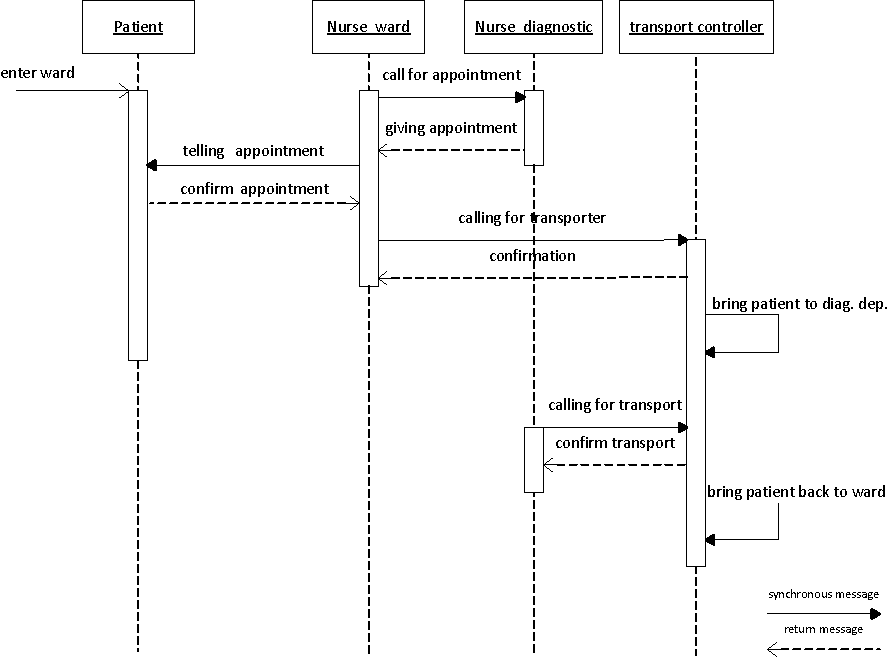
\includegraphics[width=1\textwidth]{pics/ub3/a/1a_seq} 
  \caption{Sequence diagram for scenario 1}
  \label{fig:1a_seq_dia} 
 \end{figure}
\newpage

\textbf{Statechart for patient:}
\begin{figure}[!htb]
  \centering  
  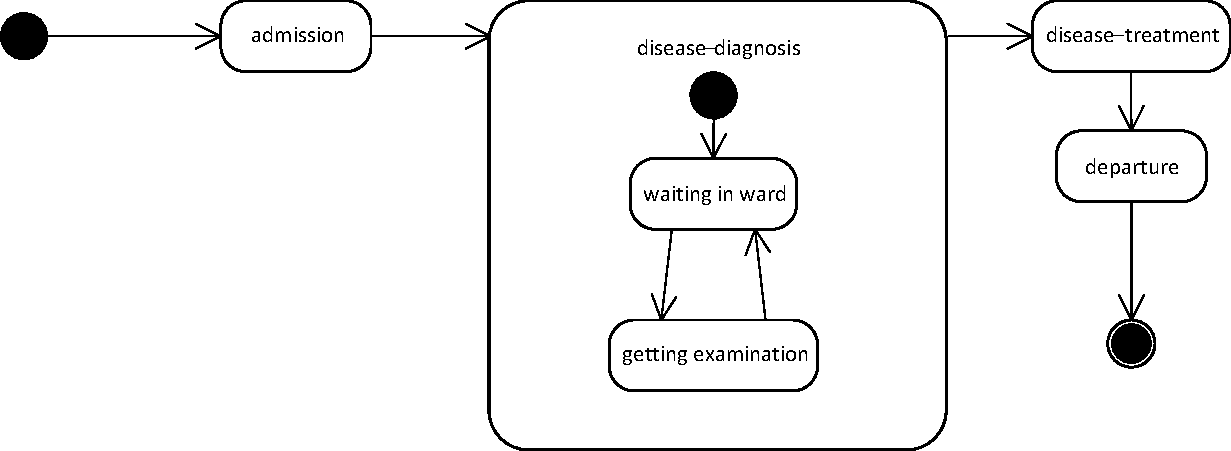
\includegraphics[width=1\textwidth]{pics/ub3/a/1a_pat} 
  \caption{Statediagram for patient}
  \label{fig:1a_pat_dia} 
 \end{figure}
 
\textbf{Statechart for nurses (ward/diagnostic):}
\begin{figure}[!htb]
  \centering  
  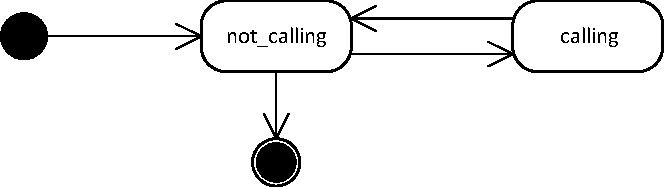
\includegraphics[width=0.7\textwidth]{pics/ub3/a/1a_nurse} 
  \caption{Statediagram for nurses}
  \label{fig:1a_nurse_dia} 
 \end{figure}
 
 \textbf{Statechart for transport controller:}
\begin{figure}[!htb]
  \centering  
  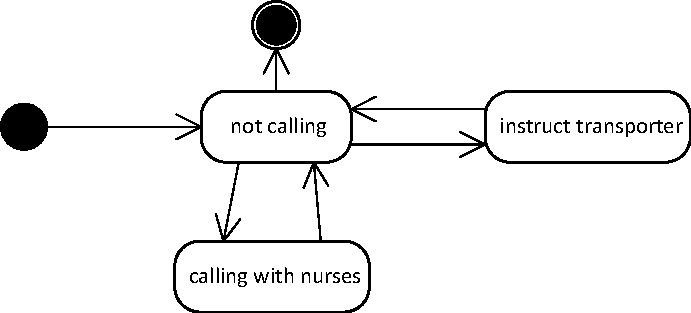
\includegraphics[width=0.7\textwidth]{pics/ub3/a/1a_contr} 
  \caption{Statediagram for transport controller}
  \label{fig:1a_contr_dia} 
 \end{figure}
 
 
 \newpage
\subsection{OP PEP}
Following sequence diagram describes the second scenario:
\begin{figure}[!htb]
  \centering  
  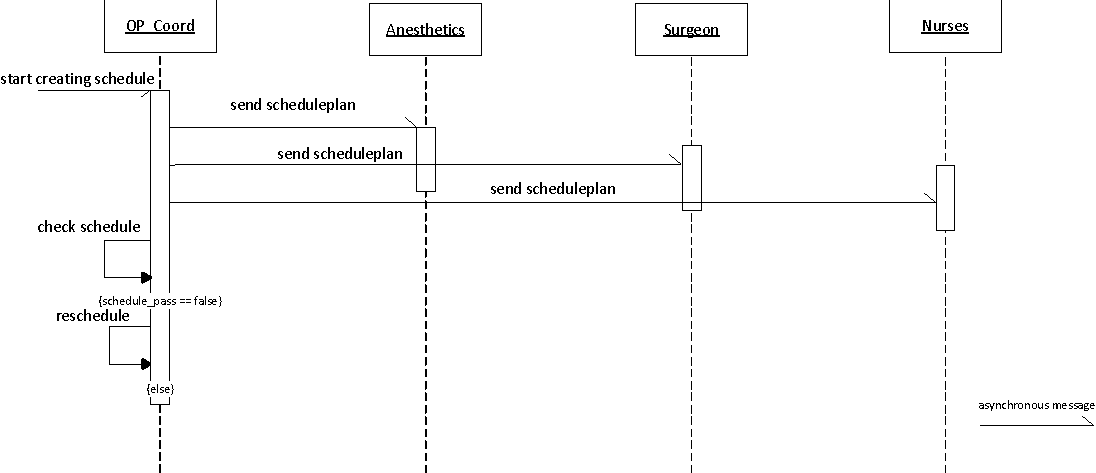
\includegraphics[width=1.1\textwidth]{pics/ub3/b/1b_seq} 
  \caption{Sequence diagram for scenario 2}
  \label{fig:1b_seq} 
 \end{figure}
 
 \textbf{Statechart for OP coordinator:}
\begin{figure}[!htb]
  \centering  
  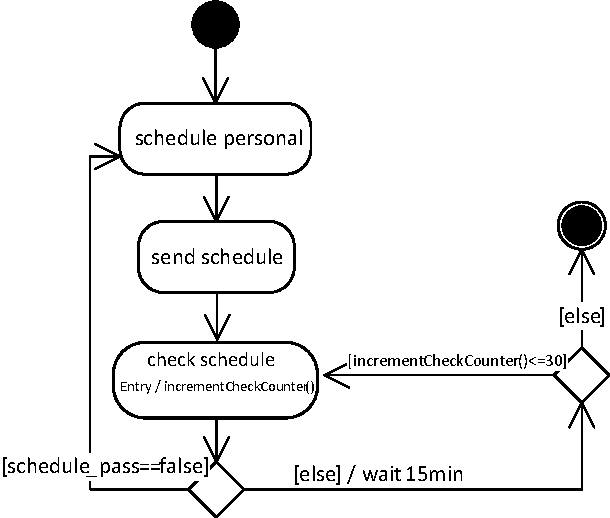
\includegraphics[width=0.7\textwidth]{pics/ub3/b/1b_orga_stat} 
  \caption{Statediagram for coordinator}
  \label{fig:1b_orga_stat} 
 \end{figure}
 
 \newpage
 
  \textbf{Statechart for surgeon:}
\begin{figure}[!htb]
  \centering  
  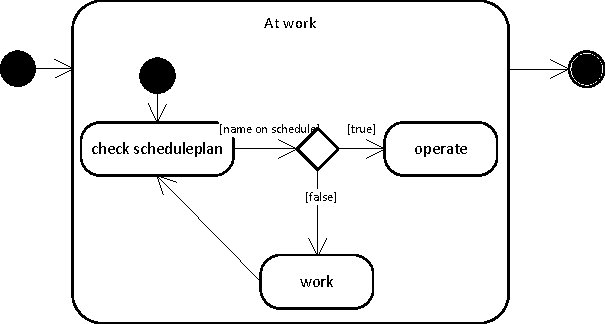
\includegraphics[width=0.7\textwidth]{pics/ub3/b/1b_chir_stat} 
  \caption{Statediagram for surgeon}
  \label{fig:1b_chir_stat} 
 \end{figure}
 
   \textbf{Statechart for anesthetist:}
\begin{figure}[!htb]
  \centering  
  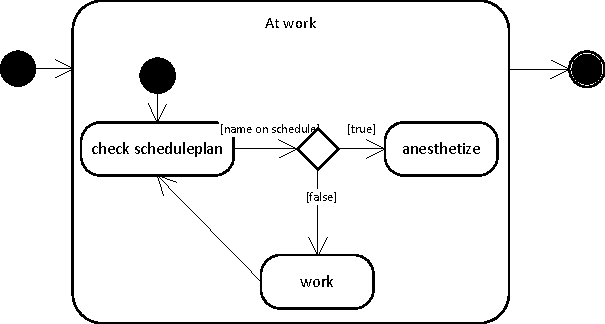
\includegraphics[width=0.7\textwidth]{pics/ub3/b/1b_anest_stat} 
  \caption{Statediagram for anesthetist}
  \label{fig:1b_anest_stat} 
 \end{figure}
 
 
    \textbf{Statechart for nurse:}
\begin{figure}[!htb]
  \centering  
  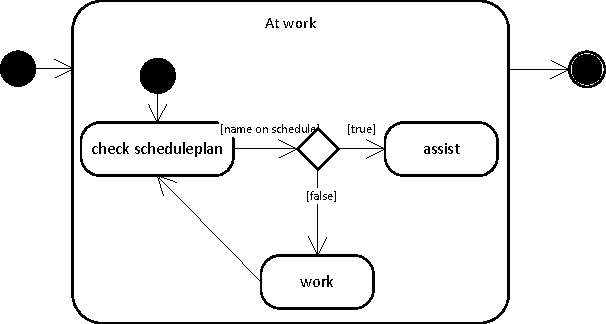
\includegraphics[width=0.7\textwidth]{pics/ub3/b/1b_nurse_stat} 
  \caption{Statediagram for nurse} 
  \label{fig:1b_nurse_stat} 
 \end{figure}

\newpage 
\textbf{Whole statechart for patient:}
\begin{figure}[!htb]
  \centering  
  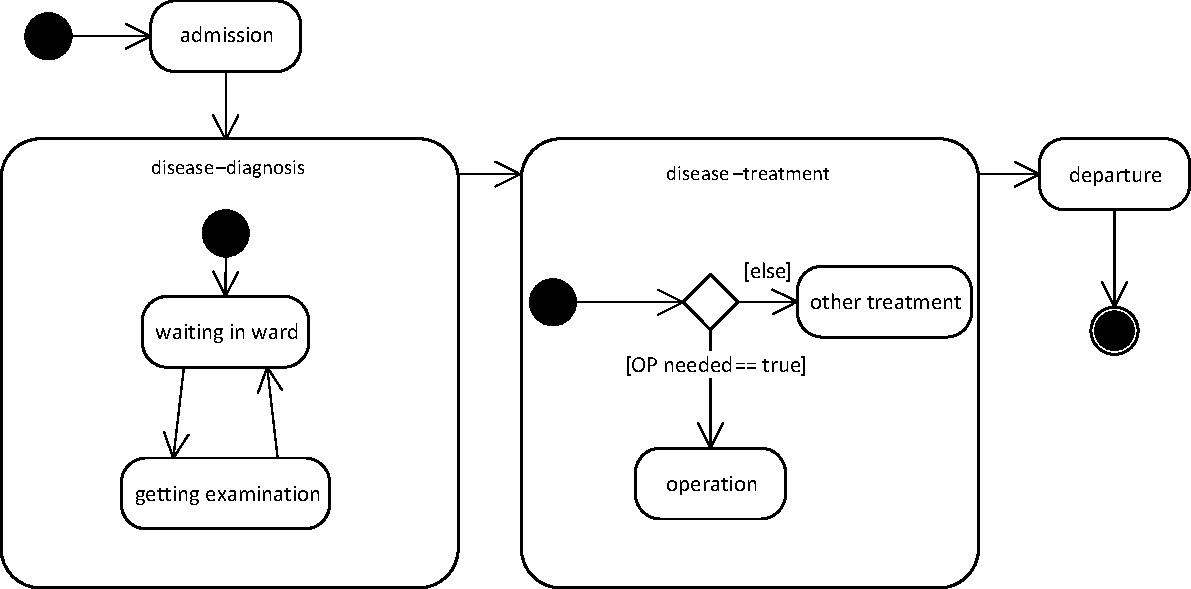
\includegraphics[width=1\textwidth]{pics/ub3/b/1b_pat_stat} 
  \caption{Statediagram for patient}
  \label{fig:1b_pat_stat} 
 \end{figure}
 
 
 \section{Simulation of the real world problem}
 \subsection{Summary of results}
The supply chain model describes in very simple terms a stilised supply chain procedure.
The key objects are the five distributors (which own one to five trucks each), the retailers and the trucks. 
The retailers comission from time to time orders for five to 20 products to one of the five distributors.
Then the trucks are loaded with the products up to their maximum capacity which is 100 products 
(however, if a truck is loaded up to 90\% it is enough for it to move out). Then the retailers which
issued the orders are successively served. If an order is issued and no truck is at the distributor,
the order is placed in a backlog; as soon as a truck arrives back at the distributor, the truck is loaded up with the goods,
which were required in the order. And the truck takes as much orders as possible out of the backlog.
\\
This simple model allows the user to manipulate several parameters (wich are
also part of the real world) like: number of trucks, max.
capacity etc. so the user can observe effects of the parameters on the behavior of the modeled system.


 
